 \documentclass{beamer}

\usetheme{MagdeburgFIN}
\usefonttheme{structurebold}
\usepackage{graphicx}
\usepackage{float}
\usepackage{url}
\usepackage{pdfpages}
\usepackage[export]{adjustbox}
\usepackage{wrapfig}
\usepackage{verbatim}

\setbeamertemplate{caption}[numbered]

\title{Build Your Own OctopusDB: Blinktopus Edition}
\author{Ali Hashaam, Ali Memon, Guzel Mussilova, Pavlo Shevchenko}
\date{July 10, 2017}
\institute{Scientific Project: Databases for Multi-Dimensional Data, Genomics and Modern Hardware}

\begin{document}

\begin{frame}[plain]
 \titlepage
\end{frame}

\begin{frame}
\frametitle{Table of Contents}
\tableofcontents
\end{frame}

\section{Motivation/Problem Statement}
% one size fits all (OLTP OLAP together)
% interactive queries (AQP part)
% HTAP freshness OLAP queries (AQP?)
\begin{frame}
\frametitle{Motivation}
\begin{enumerate}
\item{Companies need to pick only  specialized DBMSs, each tailored to their specific use-case. \\ \pause
$\Rightarrow$ Need for \emph{one size fits all system} (e.g. HTAP)}
\pause
\item{Support OLAP queries for analysis over real-time data (i.e., freshness). \\ \pause
$\Rightarrow$ Explore the techniques related to more interactive queries (e.g. \emph{Approximate Query Processing})}
\end{enumerate}
\end{frame}

\section{Background}
\begin{frame}
\frametitle{Background}
\begin{enumerate}
\item{OctopusDB}
\begin{itemize}
\item{uses logs as a primary storage}
\item{mimicks several types of systems (OLAP, OLTP, etc.) by representing them as \emph{Storage Views}}
\end{itemize}
\pause
\item{BlinkDB}
\begin{itemize}
\item{Successfully integrates AQP techniques into its architecture}
\end{itemize}
\end{enumerate}
\end{frame}
% OctopusDB (SV)
% BlinkDB (AQP)

\section{Conceptual Idea and Implementation}
% Blinktopus architecture
% Briefly Histograms (Rice rule) and HLL (Library)
\begin{frame}
\frametitle{Conceptual Idea and Implementation}
\begin{figure}
\centering
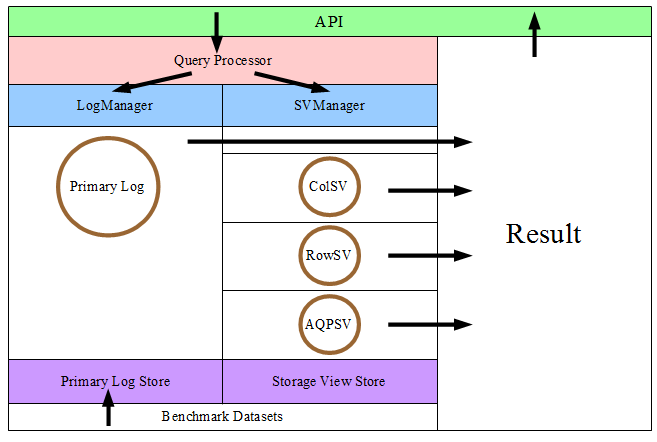
\includegraphics[scale=0.5]{img/blinktopus_architecture.png}
\caption{OctopusDB Architecture.}
\end{figure}
\end{frame}

\begin{frame}
\frametitle{Conceptual Idea and Implementation}
\textbf{Which synopses to pick?}
\begin{itemize}
\item{Equi-depth histograms}
\begin{itemize}
\item{suitable for range queries}
\item{simple to implement and interpretate}
\end{itemize}
\item{Sketches}
\begin{itemize}
\item{\emph{HyperLogLog}}
\item{\textit{DISTINCT COUNT} queries}
\item{\textit{DataSketches} library by \textit{Yahoo} \footnote{https://yahooeng.tumblr.com/post/125390948446/data-sketches}}
\end{itemize}
\end{itemize}
\end{frame}

\section{Evaluation Setup and Results}
\begin{frame}
\frametitle{Evaluation Setup}
\textbf{Machine}
\begin{itemize}
\item{CentOS Linux 7.1.1503}
\item{Java SDK 8u131-b11-linux-x64}
\item{2 Intel(r) Xeon (TM) E5-2630 v3s CPU @ 3.2GHz processors (8 cores each) and 1024 GiB memory}
\end{itemize}
\textbf{Benchmark Datasets}
\begin{itemize}
\item{TPC-H datasets (Orders and Lineitems)}
\end{itemize}
\textbf{Experiments}
\begin{enumerate}
\item{Average response time for a range query on the Orders table with various scaling factors and predicate selectivity}
\item{Average response time for a count-range query on the Orders table. Comparison with an equi-depth histogram}
\item{Average response time for a count distinct query on the Orders table. Comparison with a HLL sketch}
\end{enumerate}
\end{frame}

\begin{frame}
\frametitle{Results. Experiment 1}
\centering
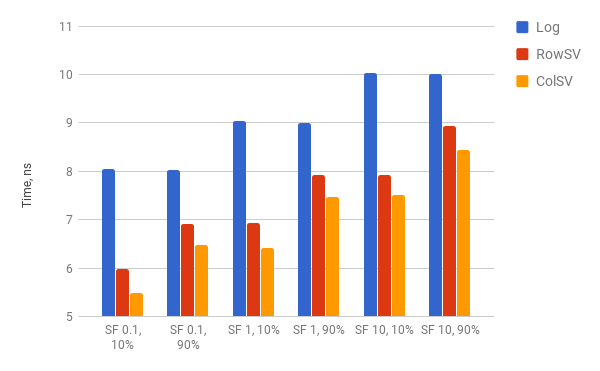
\includegraphics[scale=0.5]{img/exp1.png}
\end{frame}

\begin{frame}
\frametitle{Results. Experiment 2}
\centering
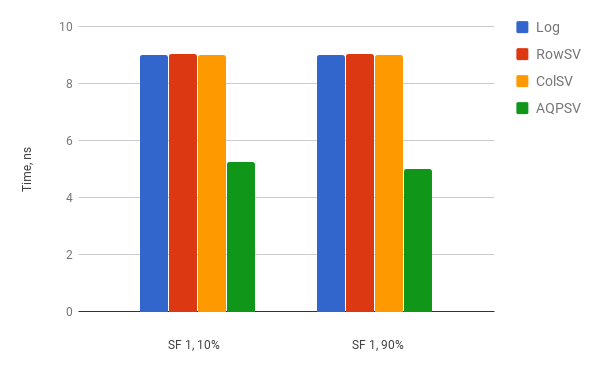
\includegraphics[scale=0.5]{img/exp2.png}
\end{frame}

\begin{frame}
\frametitle{Results. Experiment 3}
\centering
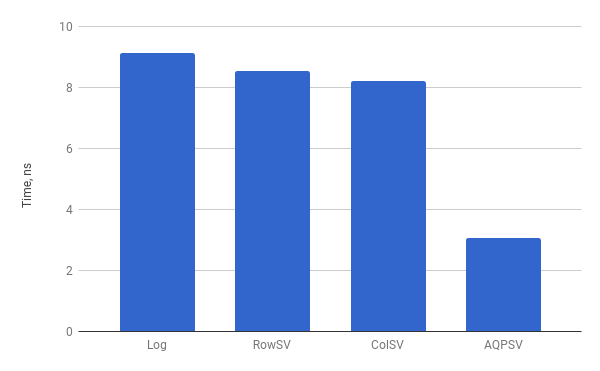
\includegraphics[scale=0.5]{img/exp3.png}
\end{frame}

\section{Related Work}
% Apache Samza, Rodent Store, Snappy Data
\begin{frame}
\frametitle{Related Work}
\begin{enumerate}
\item{Apache Samza}
\begin{itemize}
\item{logs as a primary structure}
\item{replicates logs on multiple nodes}
\end{itemize}
\item{Rodent Store}
\begin{itemize}
\item{represents data in the various physical layouts}
\item{provides DBAs a high-level interface to specify the data physical representation by means of storage algebra}
\end{itemize}
\item{Snappy Data}
\begin{itemize}
\item{AQP Support}
\item{Uses numerous types of synopses (samples, sketches)}
\item{User defines the level of accuracy and the number of column sets to approximate the results}
\end{itemize}
\end{enumerate}
\end{frame}

\section{Conclusion and Future Work}
% Challenges (memory problem)
% Conclusion from paper
% Future Work from paper
\begin{frame}
\frametitle{Conclusion}
\begin{itemize}
\item{OLAP queries can benefit from AQP techniques}
\end{itemize}
\end{frame}

\begin{frame}
\frametitle{Future Work}
\begin{itemize}
\item{optimize centralized log (e.g. log replication, garbage collection)}
\item{extend Blinktopus architecture to support transactional model}
\item{extend query classes by implementing sample-based data synopses}
\end{itemize}
\end{frame}

\section{Demonstration}

\begin{frame}
\frametitle{Thank you!}
\end{frame}

\begin{frame}
 \frametitle{Questions? Recommendations? Remarks?}
\end{frame}

\begin{frame}
\frametitle{Literature}
\begin{enumerate}
\item{Jindal, Alekh. "The mimicking octopus: Towards a one-size-fits-all database architecture." VLDB PhD Workshop. 2010.}
\item{Dittrich, Jens, and Alekh Jindal. "Towards a One Size Fits All Database Architecture." CIDR. 2011.}
\item{Jindal, Alekh. "OctopusDB: flexible and scalable storage management for arbitrary database engines." (2012).}
\item{Mozafari, Barzan, and Ning Niu. "A Handbook for Building an Approximate Query Engine." IEEE Data Eng. Bull. 38, no. 3 (2015): 3-29.}
\item{Cormode, Graham, Minos Garofalakis, Peter J. Haas, and Chris Jermaine. "Synopses for massive data: Samples, histograms, wavelets, sketches." Foundations and Trends in Databases 4, no. 1–3 (2012): 1-294.}
%%\item{https://yahooeng.tumblr.com/post/135390948446/data-sketches}
\end{enumerate}
\end{frame}

\end{document}
